% Provenance (never printed): see sources/outline_sources.md (Year 3:
% sequence stratigraphy, accommodation and supply, systems tracts,
% cyclostratigraphy). Brief: sources/book5/BRIEFS.md, ch. 16. Curves from
% figdata/bachelor-3/shelf_model.py and lr04_periodogram.py. Exercise and
% problem values in the Book 5 scratch calculator calc/ch16.py. The Varden
% basin, its shelf and its core are invented.
\chapter{Stratigrafi Sekuen}\label{ch:b3:sequence-stratigraphy}

Melintasi penampang seismik sebuah margin benua, refleksi bertumpang di atas
yang lebih tua, lalu membangun ke arah cekungan, kemudian mundur ke arah daratan, dan
pola itu berulang lebih tinggi. Setiap paket mencatat pertarungan antara
dua laju: laju ketika ruang untuk sedimen tercipta, oleh penurunan dan oleh
naiknya permukaan laut, dan laju ketika sungai mengisinya. Stratigrafi sekuen
membaca pertarungan itu dari geometri lapisan, dan \omterm{def:b3:sequence-stratigraphy:cyclo}{siklostratigrafi} membaca
jamnya dari ketebalan lapisan.

\begin{recall}
Akomodasi, eustasi, muka laut relatif, penurunan, dan cekungan sedimen
ada di volume Tahun 1, pada bab tentang diagenesis dan cekungan sedimen.
Transgresi dan regresi laut serta siklus muka laut orde pertama ada di
volume Tahun 2, pada bab tentang Bumi Fanerozoikum; parameter
Milankovitch dan presesi iklim pada bab tentang pemaksaan orbital dan
zaman es; model umur pada bab tentang arsip iklim
dan proksi. \omterm{def:b3:exploration-seismology:terminations}{Onlap}, \omterm{def:b3:exploration-seismology:terminations}{downlap}, \omterm{def:b3:exploration-seismology:terminations}{toplap}, \omterm{def:b3:exploration-seismology:terminations}{pemancungan erosional} dan
\omterm{def:b3:exploration-seismology:seismic-stratigraphy}{stratigrafi seismik} ada di Bab~\ref{ch:b3:exploration-seismology}. Deret Fourier
dan transformasi Fourier ada di buku matematika.
\end{recall}

\section{Akomodasi, pasokan dan garis pantai}\label{sec:b3:sequence-stratigraphy:shoreline}

Di setiap titik cekungan, muka laut relatif naik dengan laju $A = \dot E
+ \sigma$, yaitu laju eustatik ditambah laju penurunan (turun bila $A < 0$).
Muka laut relatif di suatu tempat ditentukan oleh permukaan laut global dan oleh
segala yang menggerakkan tanah di bawahnya: \omterm{def:b3:lithosphere-thermal-models:thermal-subsidence}{penurunan termal}, beban
sedimen dan lenturan yang ditimbulkannya, pemantulan kerak setelah lembaran
es mencair, dan dorongan lambat mantel di bawah lempeng. Muka laut relatif yang naik
menciptakan akomodasi; sedimen mengisinya. Apakah garis pantai
bergerak ke arah laut atau ke arah daratan bergantung pada keduanya, bukan
pada permukaan laut saja.
% ledger: miller20:rsl

\begin{definition}[Regresi normal dan regresi paksa]\label{def:b3:sequence-stratigraphy:regression}
Yang disebut \emph{regresi normal}\index{regresi normal} adalah gerakan garis pantai
ke arah laut selagi muka laut relatif naik: pasokan melampaui akomodasi yang
tercipta di garis pantai. Yang disebut \emph{regresi paksa}\index{regresi paksa}
adalah gerakan ke arah laut yang didorong oleh turunnya muka laut relatif:
garis pantai didorong ke arah cekungan apa pun pasokannya, dan lahan yang
ditinggalkan terpapar dan tererosi.
\end{definition}

\begin{definition}[Lintasan garis pantai]\label{def:b3:sequence-stratigraphy:trajectory}
Yang disebut \emph{lintasan garis pantai}\index{lintasan garis pantai} adalah jalur
garis pantai sepanjang waktu, digambar pada penampang kemiringan dalam kerangka
sedimen, sehingga memperlihatkan baik gerak horizontal garis pantai maupun
naik atau turunnya terhadap lapisan di bawahnya.
\end{definition}

Sebuah profil sederhana membuat pertarungan itu eksak. Di belakang garis pantai ada topset datar
selebar $W$ yang berada pada permukaan laut; di depannya terdapat foreset dengan kemiringan
$\tan\theta$ yang turun ke dasar cekungan, sedalam $D$ di bawahnya. Pasokan sedimen
$Q$ adalah volume per satuan waktu per meter garis pantai (luas per satuan waktu
pada penampang).

\begin{proposition}[Lintasan garis pantai]\label{prop:b3:sequence-stratigraphy:trajectory}
Jika muka laut relatif naik ($A \ge 0$) dan topset menumpuk secara seragam,
garis pantai bergerak dengan laju
\[
\frac{\mathrm dx_s}{\mathrm dt} = \frac{Q - AW}{D};
\]
ia maju selama $Q > AW$ dan mundur bila $AW > Q$. Jika muka laut relatif
turun ($A < 0$), topset tidak menerima apa-apa dan
\[
\frac{\mathrm dx_s}{\mathrm dt} = \frac{Q}{D} + \frac{|A|}{\tan\theta}.
\]
Dalam kedua kasus, lintasan naik atau turun pada sudut yang tangennya
$A/(\mathrm dx_s/\mathrm dt)$.
\end{proposition}

\begin{proof}
Dalam selang waktu $\mathrm dt$, topset memerlukan sedimen sebanyak $AW\,\mathrm dt$
agar tetap berada pada permukaan laut. Sisanya, $(Q - AW)\,\mathrm dt$, disebar pada foreset,
yaitu dinding setinggi $D$ yang maju sejauh $(Q - AW)\,\mathrm dt/D$; sisa negatif
berarti laut membanjiri topset lebih cepat daripada topset terisi. Ketika muka laut
turun, topset berada di atas air dan tidak menerima apa-apa, dan garis pantai
meluncur turun di sepanjang foreset lama sejauh $|A|\,\mathrm dt/\tan\theta$ tanpa
sedimen, sedangkan seluruh pasokan membangun foreset maju sejauh $Q\,\mathrm
dt/D$. Garis pantai naik sejauh $A\,\mathrm dt$ terhadap lapisan di bawahnya
selama ia bergerak sejauh $\mathrm dx_s$, dan dari sini diperoleh sudutnya.
\end{proof}

Oleh karena itu, \omterm{def:b3:sequence-stratigraphy:regression}{regresi normal} memerlukan pasokan yang lebih besar daripada akomodasi
yang tercipta pada topset, dan lintasannya naik; \omterm{def:b3:sequence-stratigraphy:regression}{regresi paksa} terjadi
apa pun pasokannya, dan lintasannya turun. Rasio kedua laju,
yang sering ditulis $A/S$, memilah pola-polanya: progradasi bila $A/S < 1$ pada
topset, agradasi di sekitar 1, dan retrogradasi di atasnya. Kurva permukaan laut yang sama
karena itu dapat menghasilkan regresi pada margin yang kaya sedimen dan
transgresi pada margin yang miskin.

\section{Geometri stratal: sekuen dan traktus sistem}\label{sec:b3:sequence-stratigraphy:sequences}

\omterm{def:b3:exploration-seismology:terminations}{Terminasi refleksi} pada Bab~\ref{ch:b3:exploration-seismology}
adalah kosakata metode ini: \omterm{def:b3:exploration-seismology:terminations}{onlap} dan \omterm{def:b3:exploration-seismology:terminations}{downlap} menandai dasar sebuah
paket, \omterm{def:b3:exploration-seismology:terminations}{toplap} dan \omterm{def:b3:exploration-seismology:terminations}{pemancungan erosional} menandai puncaknya. Dibaca pada penampang kemiringan, mereka
membagi sebuah margin menjadi paket-paket yang dibatasi oleh permukaan tanpa pengendapan atau
erosi, masing-masing mencatat satu siklus muka laut relatif.

\begin{definition}[Sekuen pengendapan dan batas sekuen]\label{def:b3:sequence-stratigraphy:sequence}
Yang disebut \emph{sekuen pengendapan}\index{sekuen pengendapan} adalah suksesi lapisan yang
berkaitan secara genetik, tanpa jeda besar di dalamnya, dibatasi di dasar
dan puncaknya oleh ketidakselarasan atau oleh keselarasan yang melanjutkannya ke
dalam cekungan. Permukaan pembatasnya adalah \emph{batas
sekuen}\index{batas sekuen}: ketidakselarasan yang terpotong oleh pemaparan dan
erosi di paparan selama turunnya muka laut relatif, beralih ke arah
cekungan menjadi keselarasan korelatif.
\end{definition}

\begin{definition}[Traktus sistem]\label{def:b3:sequence-stratigraphy:tract}
Yang disebut \emph{traktus sistem}\index{traktus sistem} adalah himpunan
sistem pengendapan (sungai, pantai, paparan, lereng) yang aktif bersama selama satu
bagian siklus muka laut relatif, dikenali dari posisinya dalam
sekuen, permukaan pembatasnya, dan pola penumpukannya. Ada empat
yang dibedakan:
\begin{itemize}
\item yang pertama, \emph{traktus sistem tahap turun}\index{traktus sistem tahap turun},
  dibangun oleh \omterm{def:b3:sequence-stratigraphy:regression}{regresi paksa} selama muka laut relatif turun:
  foreset yang bertangga turun dan terlepas dari paparan lama;
\item \emph{traktus sistem permukaan laut rendah}\index{traktus sistem permukaan laut rendah},
  dibangun oleh \omterm{def:b3:sequence-stratigraphy:regression}{regresi normal} begitu muka laut relatif mulai naik lagi,
  pada posisi garis pantai terendah: baji yang menumpuk ke atas dan menjorok ke depan;
\item \emph{traktus sistem transgresif}\index{traktus sistem transgresif},
  dibangun selama garis pantai mundur ke arah darat: satuan yang bertumpuk mundur
  dan berkeselarasan \omterm{def:b3:exploration-seismology:terminations}{onlap} di atas paparan lama;
\item \emph{traktus sistem permukaan laut tinggi}\index{traktus sistem permukaan laut tinggi},
  dibangun oleh \omterm{def:b3:sequence-stratigraphy:regression}{regresi normal} di akhir kenaikan, ketika pasokan kembali melampaui
  akomodasi: foreset yang menjorok ke depan dan \omterm{def:b3:exploration-seismology:terminations}{downlap} di atas endapan di bawahnya.
\end{itemize}
\end{definition}

\begin{definition}[Permukaan transgresif dan permukaan genang maksimum]\label{def:b3:sequence-stratigraphy:surfaces}
Yang disebut \emph{permukaan transgresif}\index{permukaan transgresif} adalah \omterm{def:b3:sequence-stratigraphy:parasequence}{permukaan
genang} signifikan pertama di atas endapan permukaan laut rendah: permukaan ini menandai
berbaliknya garis pantai dari regresi menjadi transgresi. \emph{Permukaan genang
maksimum}\index{permukaan genang maksimum} menandai posisi garis pantai yang
paling jauh ke arah darat, yaitu peralihan dari transgresi ke regresi permukaan laut tinggi;
foreset permukaan laut tinggi \omterm{def:b3:exploration-seismology:terminations}{downlap} di atasnya.
\end{definition}

\begin{definition}[Penampang termampatkan dan lembah torehan]\label{def:b3:sequence-stratigraphy:condensed}
Yang disebut \emph{penampang termampatkan}\index{penampang termampatkan} adalah interval tipis
yang diendapkan sangat lambat jauh dari garis pantai, ketika laut menggenangi paparan
dan sedimen terperangkap di dekat pantai: setebal beberapa sentimeter atau desimeter
berupa lempung, fosil, glaukonit, atau fosfat yang mungkin merekam waktu yang lama. Yang
disebut \emph{lembah torehan}\index{lembah torehan} adalah lembah sungai yang terpotong ke dalam
paparan yang tersingkap selama muka laut relatif turun, dan terisi selama
permukaan laut rendah dan transgresi berikutnya.
\end{definition}

\begin{omfigure}
\begin{tikzpicture}[font=\scriptsize, x=0.9cm, y=1.25cm, >=Stealth]
% older highstand deposits below the sequence boundary
\fill[black!10] (0,0) -- (14,0) -- (14,0.4) -- (10,0.6) -- (6,2.8) -- (0,3.0) -- cycle;
\draw[black!35] (1.5,2.0) .. controls (3.2,1.95) and (4.5,1.2) .. (8.5,0.45);
\draw[black!35] (3.5,2.93) .. controls (4.8,2.85) and (6,1.6) .. (10.5,0.42);
% falling-stage systems tract
\fill[red!25] (6.0,2.8) -- (7.4,2.25) -- (8.4,1.85) -- (9.4,1.35) -- (10.4,0.75) -- (10.6,0.58) -- (10,0.6) -- cycle;
\draw[red!60!black] (6.6,2.56) .. controls (7.0,2.4) and (7.5,1.95) .. (8.0,1.70);
\draw[red!60!black] (7.6,2.17) .. controls (8.0,2.0) and (8.5,1.45) .. (9.0,1.15);
\draw[red!60!black] (8.6,1.75) .. controls (9.0,1.55) and (9.5,0.9) .. (10.0,0.6);
% lowstand wedge
\fill[orange!40] (9.2,1.45) -- (10.4,1.5) -- (11.5,1.0) -- (12.6,0.6) -- (13.4,0.44) -- (10.6,0.58) -- (10.4,0.75) -- cycle;
% incised valley and its fill
\fill[orange!30] (2.9,2.9) .. controls (3.3,2.3) and (3.9,2.3) .. (4.3,2.86) -- cycle;
% transgressive systems tract
\fill[green!45!black!35] (11.5,1.0) -- (10.4,1.5) -- (9.2,1.45) -- (8.4,1.85) -- (7.4,2.25) -- (6.0,2.8) -- (1.0,2.97) -- (1.0,3.05) -- (6.0,2.95) -- (7.6,2.5) -- (9.4,1.75) -- (10.8,1.45) -- cycle;
% highstand systems tract
\fill[blue!22] (0,3.62) -- (7.5,3.42) -- (9.8,2.2) -- (11.2,1.22) -- (10.8,1.45) -- (9.4,1.75) -- (7.6,2.5) -- (6.0,2.95) -- (1.0,3.05) -- (0,3.07) -- cycle;
\draw[blue!60!black] (4.0,3.52) .. controls (5.0,3.45) and (5.8,3.1) .. (6.6,2.79);
\draw[blue!60!black] (5.6,3.47) .. controls (6.6,3.4) and (7.4,2.8) .. (8.2,2.26);
\draw[blue!60!black] (6.8,3.44) .. controls (7.8,3.35) and (8.8,2.4) .. (9.7,1.69);
% surfaces
\draw[red!70!black, very thick] (0,3.0) -- (2.9,2.9) .. controls (3.3,2.3) and (3.9,2.3) .. (4.3,2.86) -- (6.0,2.8) -- (7.4,2.25) -- (8.4,1.85) -- (9.2,1.45);
\draw[red!70!black, very thick, densely dashed] (9.2,1.45) -- (9.4,1.35) -- (10.4,0.75) -- (10.6,0.58) -- (14,0.4);
\draw[green!40!black, thick] (11.5,1.0) -- (10.4,1.5) -- (9.2,1.45);
\draw[blue!60!black, thick] (0,3.07) -- (1.0,3.05) -- (6.0,2.95) -- (7.6,2.5) -- (9.4,1.75) -- (10.8,1.45) -- (11.5,1.03) -- (12.6,0.63) -- (13.4,0.47) -- (14,0.43);
% labels
\node[blue!50!black] at (2.6,3.36) {permukaan laut tinggi (HST)};
\node[green!35!black, anchor=south] at (4.8,3.92) {transgresif (TST)};
\draw[green!35!black] (4.8,3.92) -- (4.4,3.01);
\node[red!60!black, anchor=west] at (10.1,2.45) {tahap turun (FSST)};
\draw[red!60!black] (10.1,2.45) -- (8.8,1.62);
\node[orange!60!black, anchor=west] at (12.2,1.55) {permukaan laut rendah (LST)};
\draw[orange!60!black] (12.2,1.55) -- (11.2,0.85);
\node[anchor=north, align=center] at (3.6,2.25) {lembah\\ torehan};
\node[red!70!black, anchor=north] at (1.4,2.95) {SB};
\node[red!70!black, anchor=north] at (12.0,0.38) {keselarasan korelatif};
\node[blue!60!black, anchor=west] at (12.7,1.1) {MFS};
\draw[blue!60!black] (12.7,1.1) -- (12.1,0.82);
\node[green!40!black, anchor=west] at (11.6,2.0) {TS};
\draw[green!40!black] (11.6,2.0) -- (10.9,1.27);
\node[blue!60!black, anchor=south] at (13.4,0.58) {termampatkan};
\node[anchor=west, black!60] at (0.2,0.35) {endapan lebih tua};
\draw[->] (11.2,3.9) -- (12.6,3.9) node[right] {ke arah cekungan};
\end{tikzpicture}

\par\smallskip{\small Anatomi \omterm{def:b3:sequence-stratigraphy:sequence}{sekuen pengendapan} pada penampang kemiringan
(skematis, skala vertikal jauh dilebih-lebihkan). \omterm{def:b3:sequence-stratigraphy:sequence}{Batas sekuen} (SB, merah)
adalah ketidakselarasan di paparan, dengan \omterm{def:b3:sequence-stratigraphy:condensed}{lembah torehan}, dan keselarasan korelatif
di cekungan (putus-putus); di sini batas itu digambar di atas endapan tahap
turun. \omterm{def:b3:sequence-stratigraphy:surfaces}{Permukaan transgresif} (TS) menutup baji permukaan laut rendah; \omterm{def:b3:sequence-stratigraphy:surfaces}{permukaan
genang maksimum} (MFS) menutup traktus transgresif yang tipis dan beralih ke arah
cekungan menjadi \omterm{def:b3:sequence-stratigraphy:condensed}{penampang termampatkan}; foreset permukaan laut tinggi \omterm{def:b3:exploration-seismology:terminations}{downlap} di atasnya.}\label{fig:b3:sequence-stratigraphy:anatomy}
\end{omfigure}

Di mana tepatnya \omterm{def:b3:sequence-stratigraphy:sequence}{batas sekuen} berada di cekungan adalah soal konvensi, dan
para penulis berbeda pendapat: sebagian menggambarnya di dasar endapan tahap turun, tempat
penurunan dimulai, sebagian lain di puncaknya, tempat penurunan berakhir, seperti pada gambar di atas.
Di paparan tidak ada keraguan: batasnya adalah permukaan pemaparan
dan erosi, dan endapan di atasnya lebih muda daripada penurunan itu.

Dibaca dari bawah ke atas di satu tempat pada paparan luar, sebuah sekuen mencatat
siklusnya: foreset permukaan laut tinggi, permukaan pemaparan, mungkin isian lembah,
\omterm{def:b3:sequence-stratigraphy:surfaces}{permukaan transgresif}, lapisan yang bertumpuk mundur, interval termampatkan di
\omterm{def:b3:sequence-stratigraphy:surfaces}{permukaan genang maksimum}, lalu foreset permukaan laut tinggi lagi. Hierarki
siklus ditentukan oleh penyebabnya: pembukaan dan penutupan samudra
untuk siklus orde pertama, perubahan volume es dan laju penyebaran dasar laut
untuk siklus yang lebih pendek, dan tektonik lokal serta pasokan untuk
semuanya.

\section{Parasekuen dan pola penumpukan}\label{sec:b3:sequence-stratigraphy:parasequences}

Di dalam \omterm{def:b3:sequence-stratigraphy:tract}{traktus sistem}, paket terkecil yang dipetakan geolog pada tebing atau
log sumur adalah satuan yang mendangkal ke atas dengan tebal beberapa meter sampai
beberapa puluh meter, ditutup oleh permukaan tempat air yang lebih dalam tiba-tiba kembali.

\begin{definition}[Parasekuen dan permukaan genang]\label{def:b3:sequence-stratigraphy:parasequence}
Yang disebut \emph{parasekuen}\index{parasekuen} adalah suksesi yang relatif selaras
yang tersusun dari lapisan-lapisan yang berhubungan secara genetik dan dibatasi permukaan genang,
dengan air yang mendangkal ke atas: di pesisir yang didominasi gelombang, lumpur lepas pantai beralih ke atas
menjadi pasir muka pantai bawah dan atas, serta gisik. Yang disebut \emph{permukaan
genang}\index{permukaan genang} adalah permukaan yang di atasnya fasies air lebih dalam
secara tiba-tiba menimpa fasies yang lebih dangkal, dengan bukti pendalaman mendadak.
\end{definition}

Satu \omterm{def:b3:sequence-stratigraphy:parasequence}{parasekuen} menjadi lebih kasar ke atas, dan log sinar gammanya, rendah pada pasir
dan tinggi pada lempung, membentuk bentuk corong yang menyempit ke atas. Cara
\omterm{def:b3:sequence-stratigraphy:parasequence}{parasekuen} dalam suatu traktus saling menumpuk menunjukkan tren garis pantai:
masing-masing dibangun lebih jauh ke arah laut daripada yang sebelumnya (progradasi),
di atas yang sebelumnya (agradasi), atau ke arah darat (retrogradasi). Log
melalui tumpukan itu memperlihatkan tren secara langsung: setiap \omterm{def:b3:sequence-stratigraphy:parasequence}{parasekuen} berakhir
dengan fasies yang lebih kasar dan lebih dangkal daripada yang di bawahnya, sama, atau lebih halus dan lebih dalam.
\omterm{def:b3:sequence-stratigraphy:tract}{Traktus sistem permukaan laut tinggi} dan permukaan laut rendah menumpuk secara progradasional atau agradasional,
\omterm{def:b3:sequence-stratigraphy:tract}{traktus sistem transgresif} menumpuk secara retrogradasional. Bab berikutnya membaca
log semacam ini fasies demi fasies.

\begin{omfigure}
\begin{tikzpicture}[font=\scriptsize, x=1cm, y=1cm]
% three logs: each parasequence a coarsening-upward wedge (grain size to the right)
% progradational
\begin{scope}[xshift=0cm]
\fill[yellow!45!brown!35] (0,0) -- (0.5,0) -- (1.4,1.1) -- (0,1.1) -- cycle;
\fill[yellow!45!brown!35] (0,1.1) -- (0.5,1.1) -- (1.8,2.2) -- (0,2.2) -- cycle;
\fill[yellow!45!brown!35] (0,2.2) -- (0.5,2.2) -- (2.2,3.3) -- (0,3.3) -- cycle;
\draw (0,0) -- (0.5,0) -- (1.4,1.1) -- (0.5,1.1) -- (1.8,2.2) -- (0.5,2.2) -- (2.2,3.3) -- (0,3.3) -- cycle;
\node[anchor=north, align=center] at (1.1,-0.1) {progradasi\\ (garis pantai bergerak ke arah laut)};
\end{scope}
% aggradational
\begin{scope}[xshift=4.2cm]
\fill[yellow!45!brown!35] (0,0) -- (0.5,0) -- (1.8,1.1) -- (0,1.1) -- cycle;
\fill[yellow!45!brown!35] (0,1.1) -- (0.5,1.1) -- (1.8,2.2) -- (0,2.2) -- cycle;
\fill[yellow!45!brown!35] (0,2.2) -- (0.5,2.2) -- (1.8,3.3) -- (0,3.3) -- cycle;
\draw (0,0) -- (0.5,0) -- (1.8,1.1) -- (0.5,1.1) -- (1.8,2.2) -- (0.5,2.2) -- (1.8,3.3) -- (0,3.3) -- cycle;
\node[anchor=north, align=center] at (1.1,-0.1) {agradasi\\ (garis pantai tetap)};
\end{scope}
% retrogradational
\begin{scope}[xshift=8.4cm]
\fill[yellow!45!brown!35] (0,0) -- (0.5,0) -- (2.2,1.1) -- (0,1.1) -- cycle;
\fill[yellow!45!brown!35] (0,1.1) -- (0.5,1.1) -- (1.8,2.2) -- (0,2.2) -- cycle;
\fill[yellow!45!brown!35] (0,2.2) -- (0.5,2.2) -- (1.4,3.3) -- (0,3.3) -- cycle;
\draw (0,0) -- (0.5,0) -- (2.2,1.1) -- (0.5,1.1) -- (1.8,2.2) -- (0.5,2.2) -- (1.4,3.3) -- (0,3.3) -- cycle;
\node[anchor=north, align=center] at (1.1,-0.1) {retrogradasi\\ (garis pantai bergerak ke arah darat)};
\end{scope}
% flooding surfaces
\foreach \s in {0,4.2,8.4} {
  \draw[omDef, thick] (\s-0.15,1.1) -- (\s+2.5,1.1);
  \draw[omDef, thick] (\s-0.15,2.2) -- (\s+2.5,2.2);
  \node[omDef, anchor=west] at (\s+2.5,1.1) {FS};
  \node[omDef, anchor=west] at (\s+2.5,2.2) {FS};
}
% grain-size axis
\draw[->] (0,3.6) -- (2.3,3.6) node[right] {lebih kasar};
\node[anchor=east] at (0,3.6) {lumpur};
\end{tikzpicture}

\par\smallskip{\small Tiga \omterm{def:b3:sequence-stratigraphy:parasequence}{parasekuen} ditumpuk dengan tiga cara, digambar sebagai
log ukuran butir (lebar ke kanan berarti lebih kasar). Setiap \omterm{def:b3:sequence-stratigraphy:parasequence}{parasekuen}
menjadi lebih kasar ke atas dari lumpur lepas pantai ke pasir muka pantai dan berakhir pada \omterm{def:b3:sequence-stratigraphy:parasequence}{permukaan
genang} (FS); bagian atas setiap \omterm{def:b3:sequence-stratigraphy:parasequence}{parasekuen} lebih kasar daripada yang di bawahnya saat tumpukan
berprogradasi, sama saat beragradasi, dan lebih halus saat
beretrogradasi.}\label{fig:b3:sequence-stratigraphy:stacking}
\end{omfigure}

\begin{inthefield}[Parasekuen di tebing gurun]
\begin{minipage}[t]{0.52\linewidth}\vspace{0pt}
Book Cliffs di Utah timur memperlihatkan endapan garis pantai Kapur Atas
sepanjang puluhan kilometer. Di Anggota Kenilworth yang ditelusuri sepanjang tebing
dari Price ke Hatch Mesa, geolog memetakan endapan dataran pesisir, muka pantai,
paparan dalam dan endapan \omterm{def:b3:sequence-stratigraphy:condensed}{lembah torehan}, serta sembilan \omterm{def:b3:sequence-stratigraphy:parasequence}{parasekuen} yang menjadi lebih kasar ke atas,
yang didominasi gelombang sampai badai, dengan tebal 7 sampai \qty{32}{m}. Ke arah
cekungan, setiap \omterm{def:b3:sequence-stratigraphy:parasequence}{parasekuen} terbagi menjadi hingga empat kumpulan lapisan kecil yang menjadi lebih kasar ke atas, dengan tebal 2 sampai
\qty{18}{m}; sebagian pasir muka pantai bertumpu pada dasar yang tajam, yang
oleh studi ini ditafsirkan sebagai endapan permukaan laut rendah.
\end{minipage}\hfill
\begin{minipage}[t]{0.44\linewidth}\vspace{0pt}
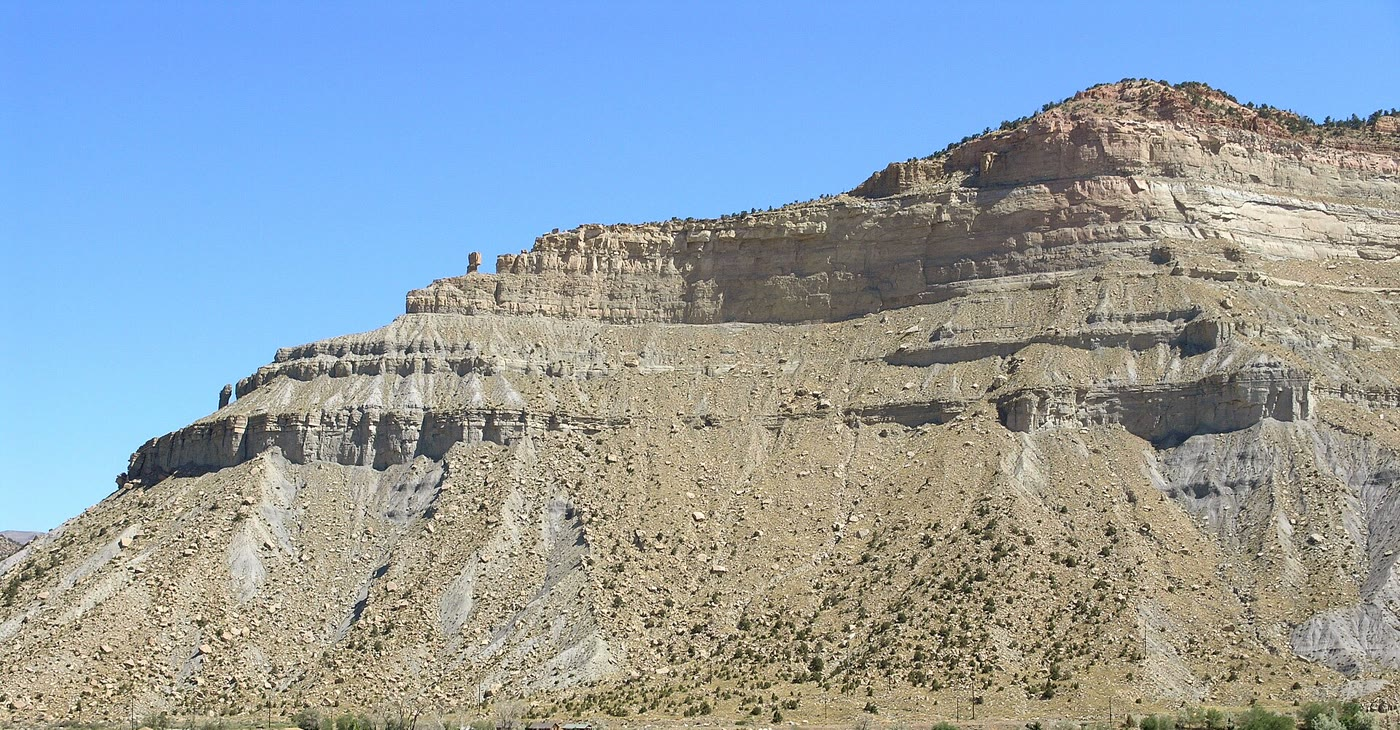
\includegraphics[width=\linewidth]{images/book5/b3-book-cliffs-helper.jpg}

{\scriptsize Book Cliffs di atas Helper, Utah: tonjolan batu pasir pucat tampak
menonjol di atas lereng batu lumpur kelabu. Foto: David Mackie, domain publik.}
\end{minipage}
\end{inthefield}
% ledger: pattison95:kenilworth, photo:b3-book-cliffs

\section{Model maju sebuah paparan}\label{sec:b3:sequence-stratigraphy:model}

Aturan pada bagian sebelumnya dapat dijalankan sebagai model. Cekungan Varden
adalah paparan rekaan: tanjakan yang miring ke arah cekungan dengan kemiringan \qty{1.5}{m/km}, yang
mengalami penurunan dengan laju $\sigma = 0.02 + x/1200$ \unit{m/ka} pada jarak $x$ (km) dari
engsel, dengan permukaan laut $E = -30\cos(2\pi t/400)$ (m, $t$ dalam ka), yang
dialiri sungai yang memasok $Q = \qty{6000}{m^3/ka}$ per meter pantai. Pada setiap langkah
setengah ribu tahun, cekungan mengalami penurunan; sedimen lalu mengisi
topset datar hingga permukaan laut, di mana pun permukaan lama terendam air, serta sebuah
foreset dengan kemiringan 0.012 di depannya, dengan garis pantai ditempatkan sehingga
volume yang ditambahkan sama dengan pasokan; lahan yang tersingkap tidak menerima apa pun dan, demi
kesederhanaan, tidak dierosi. Model dimulai pada permukaan laut rendah, setelah sebuah
baji pertama yang terbentuk pada permukaan laut konstan.

\begin{omfigure}
\begin{tikzpicture}
\begin{groupplot}[group style={group size=1 by 2, vertical sep=0.35cm, x descriptions at=edge bottom},
  omrecord, width=0.86\linewidth, xmin=0, xmax=600,
  xtick={0,100,200,300,400,500,600},
  tick label style={font=\scriptsize}, label style={font=\small}]
\nextgroupplot[height=0.2\linewidth, ylabel={$E$ (m)}, ymin=-35, ymax=35,
  ytick={-30,0,30}]
\addplot[omDef, thick, domain=0:600, samples=121] {-30*cos(deg(2*pi*x/400))};
\nextgroupplot[height=0.3\linewidth, xlabel={waktu (ka)}, ylabel={garis pantai $x_s$ (km)},
  ymin=0, ymax=60, ytick={0,20,40,60},
  scatter/classes={1={mark=*, red!70!black}, 2={mark=*, orange!80!black},
    3={mark=*, green!50!black}, 4={mark=*, blue!70!black}}]
% computed in figdata/bachelor-3/shelf_model.py
\addplot[scatter, only marks, mark size=0.9pt, scatter src=explicit symbolic]
  table[x=t, y=xs, meta=tract] {figdata/out/bachelor-3-shelf_model-shore.dat};
\node[font=\scriptsize, orange!60!black] at (axis cs:12,56) {LST};
\node[font=\scriptsize, green!40!black] at (axis cs:70,40) {TST};
\node[font=\scriptsize, blue!60!black] at (axis cs:160,6) {HST};
\node[font=\scriptsize, red!60!black] at (axis cs:300,22) {FSST};
\node[font=\scriptsize, orange!60!black] at (axis cs:415,57) {LST};
\node[font=\scriptsize, green!40!black] at (axis cs:520,45) {TST};
\node[font=\scriptsize, blue!60!black] at (axis cs:580,12) {HST};
\end{groupplot}
\end{tikzpicture}

\par\smallskip{\small Di atas, permukaan laut eustatik model Varden;
di bawah, posisi garis pantai, diwarnai menurut \omterm{def:b3:sequence-stratigraphy:tract}{traktus sistem} (permukaan laut rendah
oranye, transgresif hijau, permukaan laut tinggi biru, tahap turun merah), diklasifikasikan
hanya dari keluaran model: tahap turun saat muka laut relatif turun
di garis pantai, transgresif saat garis pantai mundur, permukaan laut rendah atau
permukaan laut tinggi saat garis pantai maju di bawah laut yang naik, setelah muka laut turun atau setelah
transgresi.}\label{fig:b3:sequence-stratigraphy:series}
\end{omfigure}

Gambar di atas mengikuti garis pantai sepanjang waktu, dan gambar di bawah
memperlihatkan endapan yang ditinggalkannya. Traktus-traktus muncul tanpa aturan tertulis ke dalam
model selain pengisian dan penurunan. Baji permukaan laut rendah di awal terletak
jauh di lepas pantai; laut yang naik mendorong garis pantai sejauh \qty{38}{km} ke arah darat pada
transgresi pertama, dan foreset permukaan laut tinggi kembali tumbuh ke arah cekungan saat kenaikan melambat.
Kemudian muka laut mulai turun: garis pantai didorong ke arah cekungan sejauh \qty{33}{km} dalam
\qty{187}{ka}, meninggalkan foreset tipis yang menurun bertahap dan paparan yang tersingkap
di belakangnya, yaitu traktus tahap turun. Baji permukaan laut rendah baru, transgresi kedua
dan permukaan laut tinggi baru menyusul. Kecepatan \omterm{def:b3:sequence-stratigraphy:regression}{regresi paksa} dalam model
sesuai dengan rumus proposisi dengan selisih beberapa persen;
di bawah laut yang naik, topset model tidak mengalami agradasi seragam, karena penurunan
makin besar ke arah cekungan, dan rumus itu hanya panduan.

\begin{omfigure}
\begin{tikzpicture}
\begin{axis}[omsection, width=0.95\linewidth, height=0.42\linewidth,
  xmin=0, xmax=70, ymin=-150, ymax=40, clip=true,
  xlabel={jarak ke arah cekungan (km)}, ylabel={elevasi sekarang (m)},
  xtick={0,10,20,30,40,50,60,70}, ytick={-150,-100,-50,0},
  tick label style={font=\scriptsize}, label style={font=\small}]
% computed in figdata/bachelor-3/shelf_model.py
\addplot[fill=black!10, draw=none] table[x=x, y=z0] {figdata/out/bachelor-3-shelf_model-surfaces.dat} -- (axis cs:120,-300) -- (axis cs:0,-300) -- cycle;
\addplot[fill=orange!45, draw=none] table[x=x, y=z] {figdata/out/bachelor-3-shelf_model-poly1.dat};
\addplot[fill=green!45!black!35, draw=none] table[x=x, y=z] {figdata/out/bachelor-3-shelf_model-poly2.dat};
\addplot[fill=blue!25, draw=none] table[x=x, y=z] {figdata/out/bachelor-3-shelf_model-poly3.dat};
\addplot[fill=red!30, draw=none] table[x=x, y=z] {figdata/out/bachelor-3-shelf_model-poly4.dat};
\addplot[fill=orange!45, draw=none] table[x=x, y=z] {figdata/out/bachelor-3-shelf_model-poly5.dat};
\addplot[fill=green!45!black!35, draw=none] table[x=x, y=z] {figdata/out/bachelor-3-shelf_model-poly6.dat};
\addplot[fill=blue!25, draw=none] table[x=x, y=z] {figdata/out/bachelor-3-shelf_model-poly7.dat};
\addplot[black!45, very thin] table[x=x, y=z40] {figdata/out/bachelor-3-shelf_model-surfaces.dat};
\addplot[black!45, very thin] table[x=x, y=z80] {figdata/out/bachelor-3-shelf_model-surfaces.dat};
\addplot[black!45, very thin] table[x=x, y=z120] {figdata/out/bachelor-3-shelf_model-surfaces.dat};
\addplot[black!45, very thin] table[x=x, y=z160] {figdata/out/bachelor-3-shelf_model-surfaces.dat};
\addplot[black!45, very thin] table[x=x, y=z240] {figdata/out/bachelor-3-shelf_model-surfaces.dat};
\addplot[black!45, very thin] table[x=x, y=z280] {figdata/out/bachelor-3-shelf_model-surfaces.dat};
\addplot[black!45, very thin] table[x=x, y=z320] {figdata/out/bachelor-3-shelf_model-surfaces.dat};
\addplot[black!45, very thin] table[x=x, y=z360] {figdata/out/bachelor-3-shelf_model-surfaces.dat};
\addplot[black!45, very thin] table[x=x, y=z440] {figdata/out/bachelor-3-shelf_model-surfaces.dat};
\addplot[black!45, very thin] table[x=x, y=z480] {figdata/out/bachelor-3-shelf_model-surfaces.dat};
\addplot[black!45, very thin] table[x=x, y=z520] {figdata/out/bachelor-3-shelf_model-surfaces.dat};
\addplot[black!45, very thin] table[x=x, y=z560] {figdata/out/bachelor-3-shelf_model-surfaces.dat};
\addplot[black, thin] table[x=x, y=z600] {figdata/out/bachelor-3-shelf_model-surfaces.dat};
\addplot[black, only marks, mark=*, mark size=0.5pt] table[x=xs, y=zfinal] {figdata/out/bachelor-3-shelf_model-shore.dat};
\node[font=\scriptsize, blue!50!black] at (axis cs:6,4) {HST};
\node[font=\scriptsize, green!30!black] at (axis cs:12,-22) {TST};
\node[font=\scriptsize, red!60!black] at (axis cs:35,-25) {FSST};
\node[font=\scriptsize, orange!60!black] at (axis cs:57.5,-60) {LST};
\node[font=\scriptsize, green!30!black] at (axis cs:36,2) {TST};
\node[font=\scriptsize, blue!50!black] at (axis cs:8,26) {HST};
\end{axis}
\end{tikzpicture}

\par\smallskip{\small Paparan Varden setelah \qty{600}{ka}, dalam posisi
kini (skala vertikal dibesar-besarkan sekitar 170 kali). Warna menunjukkan
\omterm{def:b3:sequence-stratigraphy:tract}{traktus sistem}: permukaan laut rendah oranye, transgresif hijau, permukaan laut tinggi biru,
tahap turun merah; abu-abu menunjukkan tanjakan yang lebih tua dan baji pertama. Garis tipis
adalah dasar laut setiap \qty{40}{ka}; titik hitam menelusuri garis pantai setiap
\qty{2}{ka}. Dihitung dengan model maju pada
teks.}\label{fig:b3:sequence-stratigraphy:section}
\end{omfigure}


Muka laut relatif mulai turun di garis pantai beberapa ribu tahun
setelah permukaan laut eustatik tinggi, karena penurunan lebih dulu harus diatasi,
dan berakhir beberapa ribu tahun sebelum permukaan laut eustatik rendah. Turunnya muka laut di
garis pantai dengan demikian berlangsung kurang dari separuh siklus eustatik, dan
makin pendek makin cepat cekungan itu turun.

Model semacam ini adalah uji yang jujur bagi suatu interpretasi, dan juga menunjukkan
batasnya. Penampang yang sama dapat dibangun dari sejarah yang berbeda: muka laut
turun lebih cepat dengan pasokan lebih sedikit, atau turun lebih lambat dengan pasokan lebih banyak, atau perubahan penurunan
ketimbang muka laut, karena geometrinya hanya merekam muka laut relatif
dan pasokan. Bagan global siklus muka laut yang disusun dari margin pada
tahun 1970-an dan 1980-an menetapkan waktu banyak fase muka laut turun yang sejak itu
sebagian besar dikukuhkan pengeboran untuk bagian Kapur Akhir hingga Miosen, tetapi amplitudonya,
seperti turunnya muka laut sebesar \qty{160}{m} pada Oligosen tengah, terlalu besar
dengan faktor 2 hingga 3. Amplitudo eustatik kini diambil dari isotop oksigen dan
dari sumur hasil backstripping, dan sekuen sebuah margin dibaca terlebih dahulu
sebagai rekaman lokal.
% ledger: miller20:epr, miller20:rsl

\section{Siklostratigrafi}\label{sec:b3:sequence-stratigraphy:cyclo}

Banyak suksesi berulang pada interval ketebalan yang teratur: pasangan
napal dan batu gamping, berkas lima pasangan, kumpulan berkas yang lebih besar. Jika
pengulangan itu diatur oleh parameter Milankovitch, ketebalan
siklus-siklus itu berubah menjadi waktu.

\begin{definition}[Siklostratigrafi dan penalaan astronomis]\label{def:b3:sequence-stratigraphy:cyclo}
\emph{Siklostratigrafi}\index{siklostratigrafi} mengidentifikasi dan mengukur
siklus teratur dalam suksesi sedimen dan menafsirkannya sebagai rekaman
pemaksaan periodik, terutama variasi orbit dan sumbu rotasi Bumi.
\emph{Penalaan astronomis}\index{penalaan astronomis} memberi umur pada suatu suksesi
dengan mencocokkan siklusnya satu per satu dengan deret astronomis hasil hitungan
(eksentrisitas, obliquitas, presesi, atau insolasi), yang mengubah
siklus itu menjadi model umur.
\end{definition}

Periode hasil hitungan berasal dari solusi gerak Tata Surya.
Eksentrisitas orbit Bumi memiliki suku utama \qty{405}{ka}, dan
empat suku di sekitar \qty{100}{ka} (95, 99, 124 dan \qty{131}{ka});
obliquitas memiliki suku utama \qty{41.0}{ka} dengan suku yang lebih kecil pada 39.6 dan
\qty{53.7}{ka}. Presesi iklim menggabungkan presesi sumbu
dengan gerak perihelion, pada frekuensi $p_0 + g_i$, dengan $p_0 =
50.47''$ per tahun dan $g_i$ adalah frekuensi orbit planet; periode utamanya
adalah 23.7, 22.4, 19.1 dan \qty{19.0}{ka}.
Suku \qty{405}{ka} paling stabil dan berfungsi sebagai metronom untuk suksesi yang lebih tua.
% ledger: la04:eccentricity, la04:obliquity, la04:precession

\begin{omfigure}
\begin{tikzpicture}
\begin{groupplot}[group style={group size=2 by 1, horizontal sep=0.5cm, y descriptions at=edge left},
  omrecord, width=0.52\linewidth, height=0.33\linewidth,
  xmin=0, xmax=0.06, ymin=0, ymax=1.18, clip=false,
  xtick={0,0.02,0.04,0.06}, xticklabels={0,0.02,0.04,0.06}, scaled x ticks=false,
  ytick={0,0.5,1}, title style={font=\small},
  tick label style={font=\scriptsize}, label style={font=\small},
  xlabel={frekuensi (siklus per ka)}]
\nextgroupplot[title={(a) 0 hingga \qty{1000}{ka}}, ylabel={daya relatif}]
\draw[black!40, densely dotted] (axis cs:0.01,0) -- (axis cs:0.01,1.05);
\draw[black!40, densely dotted] (axis cs:0.0244,0) -- (axis cs:0.0244,1.05);
\draw[black!40, densely dotted] (axis cs:0.0429,0) -- (axis cs:0.0429,1.05);
\draw[black!40, densely dotted] (axis cs:0.0526,0) -- (axis cs:0.0526,1.05);
\node[font=\scriptsize, anchor=south] at (axis cs:0.01,1.05) {100};
\node[font=\scriptsize, anchor=south] at (axis cs:0.0244,1.05) {41};
\node[font=\scriptsize, anchor=south] at (axis cs:0.0429,1.05) {23};
\node[font=\scriptsize, anchor=south] at (axis cs:0.0526,1.05) {19};
% computed in figdata/bachelor-3/lr04_periodogram.py
\addplot[omDef, thick] table[x=f, y=p] {figdata/out/bachelor-3-lr04_periodogram-young.dat};
\nextgroupplot[title={(b) 1250 hingga \qty{2500}{ka}}]
\draw[black!40, densely dotted] (axis cs:0.01,0) -- (axis cs:0.01,1.05);
\draw[black!40, densely dotted] (axis cs:0.0244,0) -- (axis cs:0.0244,1.05);
\draw[black!40, densely dotted] (axis cs:0.0429,0) -- (axis cs:0.0429,1.05);
\draw[black!40, densely dotted] (axis cs:0.0526,0) -- (axis cs:0.0526,1.05);
\node[font=\scriptsize, anchor=south] at (axis cs:0.01,1.05) {100};
\node[font=\scriptsize, anchor=south] at (axis cs:0.0244,1.05) {41};
\node[font=\scriptsize, anchor=south] at (axis cs:0.0429,1.05) {23};
\node[font=\scriptsize, anchor=south] at (axis cs:0.0526,1.05) {19};
\addplot[omDef, thick] table[x=f, y=p] {figdata/out/bachelor-3-lr04_periodogram-old.dat};
\end{groupplot}
\end{tikzpicture}

\par\smallskip{\small \omterm{def:b3:sequence-stratigraphy:periodogram}{Periodogram} dari stack isotop oksigen bentik LR04
dalam dua jendela (terdetrend, taper Hann, dinormalisasi terhadap puncak terbesar);
garis titik-titik menandai periode 100, 41, 23 dan \qty{19}{ka}. (a) Satu juta tahun
terakhir: pita \qty{100}{ka} mendominasi. (b) Dari 2.5 hingga
\qty{1.25}{Ma}: obliquitas \qty{41}{ka} mendominasi.}\label{fig:b3:sequence-stratigraphy:periodogram}
\end{omfigure}
% ledger: data:lr04, lr04:tuning

\begin{definition}[Periodogram]\label{def:b3:sequence-stratigraphy:periodogram}
Yang disebut \emph{periodogram}\index{periodogram} dari deret $y_0, \dots, y_{N-1}$
yang diambil sampelnya dengan langkah $\Delta$ (dalam waktu atau kedalaman), setelah penghilangan rata-rata
dan tren serta perkalian dengan taper $w_k$, adalah
\[
P(f_j) = \Bigl|\sum_{k=0}^{N-1} w_k y_k\, e^{-2\pi i f_j k\Delta}\Bigr|^2,
\qquad f_j = \frac{j}{N\Delta},\ j = 1, \dots, \frac N2:
\]
yaitu daya deret pada setiap frekuensi $f_j$, kuadrat modulus
transformasi Fourier diskritnya.
\end{definition}

Dua bilangan membatasi apa yang dapat dilihat \omterm{def:b3:sequence-stratigraphy:periodogram}{periodogram}. Langkah frekuensinya, $1/(N\Delta)$,
merupakan kebalikan panjang rekaman, dan itulah resolusinya: dua periode yang frekuensinya
berselisih lebih kecil dari itu tidak dapat dipisahkan. Frekuensi tertingginya, frekuensi Nyquist $1/(2\Delta)$,
dicapai dengan dua sampel per siklus; siklus yang lebih pendek tidak hilang melainkan
terlipat menjadi siklus semu yang lebih panjang. Taper, di sini jendela Hann,
memperhalus ujung-ujung deret agar puncak yang kuat
tidak membocorkan daya ke seluruh spektrum.


\omterm{def:b3:sequence-stratigraphy:periodogram}{Periodogram} di atas adalah contoh kerja. Dalam satu juta tahun terakhir, puncak terkuat
jatuh pada pita \qty{100}{ka} (pada \qty{91}{ka} pada kisi frekuensi
rekaman \qty{1000}{ka}, dengan tetangganya 100 dan \qty{83}{ka}),
obliquitas memiliki sepertiga dayanya dan presesi beberapa persen;
antara 2.5 dan \qty{1.25}{Ma} obliquitas membawa rekaman dan
pita \qty{100}{ka} memiliki seperenam dayanya. Ada satu kehati-hatian yang sudah tertanam dalam
data: skala waktu LR04 sendiri diperoleh dengan menala stack ke
model es sederhana yang digerakkan oleh insolasi musim panas pada \ang{65}\,LU,
dibatasi oleh laju sedimentasi bertumpuk untuk mencegah penalaan berlebih, sehingga
menemukan periode orbit di dalamnya sebagian melingkar. Uji yang tidak melingkar
adalah yang dilakukan dalam kedalaman, sebelum penalaan apa pun: jika rasio ketebalan siklus
sama dengan rasio periode orbit, pemaksaannya terbukti, dan ketebalan itu memberi
laju sedimentasi.
% ledger: lr04:tuning, la04:obliquity

\begin{method}[Laju sedimentasi dari ketebalan siklus]\label{met:b3:sequence-stratigraphy:cycles}
\begin{enumerate}
\item hitung \omterm{def:b3:sequence-stratigraphy:periodogram}{periodogram} deret dalam kedalaman, dengan resolusinya
  $1/L$ untuk bagian sepanjang $L$ dan batas Nyquistnya $1/(2\Delta z)$;
\item daftarkan panjang gelombang dari puncak-puncak signifikan, $\lambda = 1/f$;
\item bandingkan rasionya dengan rasio periode orbit (405 : 100 : 41
  : 23, atau 21 untuk presesi rata-rata); kecocokan tiga puncak adalah
  argumen yang kuat, satu puncak saja belum cukup;
\item bagi setiap panjang gelombang dengan periodenya: hasil baginya, yang seharusnya
  sama, memberi laju sedimentasi.
\end{enumerate}
\end{method}

Laju sedimentasi yang diperoleh dengan cara ini adalah rata-rata sepanjang siklus dan
mengandaikan laju yang tetap: perubahan laju di dalam bagian akan meregangkan
puncak, dan hiatus diam-diam menghilangkan siklus. Karena itu, suksesi panjang
ditala siklus demi siklus terhadap deret hitungan, dimulai dari siklus \qty{405}{ka}
lebih dahulu, lalu diperiksa terhadap umur radiometrik bila lapisan vulkanik memungkinkan.

\section{Latihan}

\begin{exercise}[$\star$]\label{exo:b3:sequence-stratigraphy:1}
Pada suatu titik di paparan, permukaan laut eustatik naik \qty{0.5}{m/ka} dan
cekungan turun \qty{0.1}{m/ka}. Hitung laju kenaikan permukaan laut relatif
dan akomodasi yang terbentuk dalam \qty{20}{ka}. Berapa laju relatif
jika permukaan laut turun \qty{0.3}{m/ka} sebagai gantinya?
\end{exercise}

\begin{exercise}[$\star$]\label{exo:b3:sequence-stratigraphy:2}
Untuk setiap kasus, sebutkan \omterm{def:b3:sequence-stratigraphy:tract}{traktus sistem} yang sedang terbentuk: (a) muka laut relatif
turun, garis pantai bergerak ke arah laut; (b) muka laut relatif naik, garis pantai
bergerak ke arah darat; (c) muka laut relatif naik perlahan di akhir
siklus, garis pantai bergerak ke arah laut dan foreset mengalami \omterm{def:b3:exploration-seismology:terminations}{downlap} ke
\omterm{def:b3:sequence-stratigraphy:surfaces}{permukaan genang maksimum}; (d) muka laut relatif baru saja mulai naik setelah
turun, dan garis pantai masih bergerak ke arah laut.
\end{exercise}

\begin{exercise}[$\star$]\label{exo:b3:sequence-stratigraphy:3}
Log sumur memperlihatkan tiga \omterm{def:b3:sequence-stratigraphy:parasequence}{parasekuen}, masing-masing makin kasar ke atas. Bagian atas dari
ketiganya, dari yang terbawah, berupa pasir halus, pasir sedang, dan pasir kasar dengan
laminasi gisik. Sebutkan pola \omterm{def:b3:exploration-seismology:stack}{stacking}, pergerakan garis pantai, dan
\omterm{def:b3:sequence-stratigraphy:tract}{traktus sistem} yang mungkin menjadi bagiannya. Apa arti urutan sebaliknya?
\end{exercise}

\begin{exercise}[$\star$]\label{exo:b3:sequence-stratigraphy:4}
Sebuah tebing memperlihatkan pasangan napal dan batu gamping yang dikelompokkan dalam bundel berisi lima; satu
bundel setebal \qty{1.6}{m}. Tafsirkan pasangan lapisan dan bundel itu dengan
periode orbit, dan hitung laju sedimentasi dari bundel-bundel tersebut.
\end{exercise}

\begin{exercise}[$\star\star$]\label{exo:b3:sequence-stratigraphy:5}
Sebuah paparan memiliki topset lebar \qty{20}{km}, foreset setinggi \qty{50}{m}, dan
pasokan sebesar \qty{4000}{m^3/ka} per meter pantai; muka laut relatif naik
dengan laju \qty{0.15}{m/ka}. Hitung kecepatan garis pantai. Pada laju naik berapa
garis pantai tetap diam?
\end{exercise}

\begin{exercise}[$\star\star$]\label{exo:b3:sequence-stratigraphy:6}
Paparan yang sama kini mengalami muka laut relatif turun dengan laju \qty{0.2}{m/ka};
kemiringan foreset 0.01. Hitung kecepatan \omterm{def:b3:sequence-stratigraphy:regression}{regresi paksa} dan bagian dari kecepatan itu
yang disebabkan oleh penurunan muka laut saja.
\end{exercise}

\begin{exercise}[$\star\star$]\label{exo:b3:sequence-stratigraphy:7}
Muka laut relatif naik dengan laju \qty{0.4}{m/ka} di atas topset lebar \qty{25}{km}.
Di bawah pasokan berapa garis pantai mundur? Dengan pasokan
\qty{6000}{m^3/ka} per meter dan muka pantai yang hanya setinggi \qty{10}{m}, seberapa
cepat garis pantai itu mundur?
\end{exercise}

\begin{exercise}[$\star\star$]\label{exo:b3:sequence-stratigraphy:8}
Suku-suku eksentrisitas 94.9 dan \qty{123.9}{ka}, serta suku 94.9 dan
\qty{98.9}{ka}: berapa lama rekaman dibutuhkan untuk memisahkan tiap pasangan dalam
\omterm{def:b3:sequence-stratigraphy:periodogram}{periodogram}? Dapatkah rekaman \qty{600}{ka} melakukannya?
\end{exercise}
% ledger: la04:eccentricity

\begin{exercise}[$\star\star$]\label{exo:b3:sequence-stratigraphy:9}
Dalam sebuah inti, 20 siklus obliquitas (masing-masing \qty{40.98}{ka}) menempati
\qty{16.4}{m}. Hitung laju sedimentasi, dan waktu antara dua lapisan abu yang
berjarak \qty{3.1}{m} dalam interval yang sama.
\end{exercise}
% ledger: la04:obliquity

\begin{exercise}[$\star\star\star$]\label{exo:b3:sequence-stratigraphy:10}
Hitung sudut \omterm{def:b3:sequence-stratigraphy:trajectory}{lintasan garis pantai} (a) pada \omterm{def:b3:sequence-stratigraphy:regression}{regresi paksa} dengan laju \qty{200}{m/ka}
dengan muka laut relatif turun \qty{0.4}{m/ka}, (b) pada \omterm{def:b3:sequence-stratigraphy:regression}{regresi normal} dengan laju
\qty{50}{m/ka} dengan muka laut relatif naik \qty{0.2}{m/ka}. Mengapa sudut yang hanya
sepecahan derajat mudah terlihat pada
penampang seismik dan sulit terlihat pada tebing?
\end{exercise}

\begin{exercise}[$\star\star\star$]\label{exo:b3:sequence-stratigraphy:11}
Konstanta presesi adalah $p_0 = 50.467718''$ per tahun dan empat frekuensi planet
adalah $g_5 = 4.257564$, $g_2 = 7.456665$, $g_4 = 17.910194$ dan
$g_3 = 17.366595''$ per tahun. Hitung periode presesi iklim
$1\,296\,000''/(p_0 + g_i)$. Periksa bahwa $g_2 - g_5$ dan $g_4 - g_5$ menghasilkan
suku eksentrisitas 405 dan \qty{95}{ka}.
\end{exercise}
% ledger: la04:precession, la04:eccentricity

\begin{exercise}[$\star\star\star$]\label{exo:b3:sequence-stratigraphy:12}
Dua cekungan merekam kenaikan muka laut relatif yang sama, \qty{0.3}{m/ka}, selama
\qty{100}{ka}. Di cekungan pertama, eustasi naik dengan \qty{0.25}{m/ka} dan cekungan
itu mengalami penurunan dengan \qty{0.05}{m/ka}; di cekungan kedua, eustasi naik dengan
\qty{0.1}{m/ka} dan cekungan itu mengalami penurunan dengan \qty{0.2}{m/ka}. Tunjukkan bahwa kedua
penampang dapat identik. Pengamatan tambahan apa yang membedakan
kedua riwayat tersebut?
\end{exercise}

\section{Soal: Permukaan laut cekungan Varden}

\begin{problem}[{Soal akhir pekan --- akomodasi, lintasan garis pantai
dan traktus sistem model paparan Varden, serta jam dari sebuah inti}]
\label{pb:b3:sequence-stratigraphy:1}
Paparan Varden pada bab ini mengalami penurunan dengan laju $\sigma = 0.02 + x/1200$
(\unit{m/ka}, $x$ dalam km), di bawah muka laut $E = -30\cos(2\pi t/400)$ (m,
$t$ dalam ka), dengan pasokan \qty{6000}{m^3/ka} per meter pantai dan
kemiringan foreset 0.012. Model ini memberikan, setiap \qty{50}{ka}, muka laut
$E$, posisi garis pantai $x_s$, laju kenaikan muka laut relatif di
garis pantai $A$ dan tinggi foreset $D$:

\begin{center}\small
\begin{tabular}{rrrrr|rrrrr}
$t$ & $E$ & $x_s$ & $A$ & $D$ & $t$ & $E$ & $x_s$ & $A$ & $D$\\
(ka) & (m) & (km) & (m/ka) & (m) & (ka) & (m) & (km) & (m/ka) & (m)\\\hline
50 & $-21.2$ & 33.5 & 0.381 & -- & 350 & $-21.2$ & 44.6 & $-0.276$ & 25.3\\
100 & 0.0 & 15.7 & 0.504 & -- & 400 & $-30.0$ & 51.3 & 0.063 & 81.6\\
150 & 21.2 & 12.8 & 0.364 & 21.1 & 450 & $-21.2$ & 52.7 & 0.397 & 99.2\\
200 & 30.0 & 16.8 & 0.034 & 41.1 & 500 & 0.0 & 40.4 & 0.525 & --\\
250 & 21.2 & 24.0 & $-0.293$ & 45.4 & 550 & 21.2 & 22.9 & 0.372 & --\\
300 & 0.0 & 32.9 & $-0.424$ & 35.7 & 600 & 30.0 & 28.2 & 0.043 & 13.4\\
\end{tabular}
\end{center}
(Tanda strip menandai garis pantai yang mundur di atas dataran pesisir yang datar, tempat
tidak ada foreset yang terbentuk.)

\medskip\noindent\textbf{Bagian I --- Akomodasi.}
\begin{enumerate}
\item Hitung laju eustatik terbesar dan kapan terjadinya.
\item Hitung laju penurunan di engsel, pada \qty{20}{km} dan \qty{50}{km}, serta
  di tepi model, \qty{120}{km}.
\item Garis pantai berada dekat \qty{17.5}{km} pada saat muka laut tinggi. Kapan
  muka laut relatif mulai turun di sana?
\item Garis pantai mencapai sekitar \qty{50}{km} dekat saat muka laut rendah. Kapan
  muka laut relatif berhenti turun di sana?
\item Berapa lama penurunan relatif di garis pantai berlangsung, dibandingkan dengan
  penurunan eustatik \qty{200}{ka}? Mengapa lebih singkat?
\item Berapa besar akomodasi yang dihasilkan penurunan saja dalam satu siklus pada
  \qty{30}{km}? Bandingkan dengan rentang eustatik.
\end{enumerate}

\medskip\noindent\textbf{Bagian II --- Garis pantai.}
\begin{enumerate}[resume]
\item Baca tabel: pada rentang waktu mana garis pantai bergerak ke arah laut,
  dan pada rentang mana ke arah darat?
\item Sebuah topset muka laut tinggi selebar \qty{15}{km} teragradasi dengan laju \qty{0.30}{m/ka}
  di depan foreset setinggi \qty{40}{m}. Hitung kecepatan
  garis pantai dengan proposisi bab ini.
\item Pada topset itu, pada laju naik berapa garis pantai akan berhenti?
\item Pada \qty{300}{ka}, hitung kecepatan \omterm{def:b3:sequence-stratigraphy:regression}{regresi paksa} dari
  tabel. Model memberikan \qty{204}{m/ka}: bandingkan.
\item Di antara dua suku, mana yang mendominasi: pasokan sedimen atau penurunan muka laut?
\item Lintasan turun dari \qty{16.3}{m} pada \qty{17.4}{km}
  (\qty{204.5}{ka}) ke \qty{-42.7}{m} pada \qty{50.7}{km}
  (\qty{391.5}{ka}), dalam elevasi sekarang. Hitung gradien rata-ratanya.
  Dari penurunan yang dialami tiap titik sejak itu, tunjukkan mengapa turunnya lintasan
  hampir sama dengan penurunan eustatik \qty{59.7}{m}.
\end{enumerate}

\medskip\noindent\textbf{Bagian III --- Traktus sistem.}
\begin{enumerate}[resume]
\item Dari tabel, tentukan \omterm{def:b3:sequence-stratigraphy:tract}{traktus sistem} untuk setiap waktu dari 150 hingga
  \qty{600}{ka}.
\item Model menempatkan awal tahap turun pada \qty{204.5}{ka}
  dan berakhirnya pada \qty{391.5}{ka}: periksa keduanya terhadap pertanyaan 3 dan 4.
\item Di mana \omterm{def:b3:sequence-stratigraphy:sequence}{batas sekuen} terbentuk dalam model ini, di paparan dan
  di cekungan? Model tidak mengalami erosi: apa yang akan diperlihatkan paparan nyata?
\item Transgresi kedua berakhir pada \qty{559}{ka} dengan garis pantai di
  \qty{18.5}{km}. Hitung laju rata-ratanya dari awalnya di \qty{52.8}{km} pada
  \qty{439.5}{ka}. Permukaan apa yang terbentuk pada akhirnya?
\item Mengapa \omterm{def:b3:sequence-stratigraphy:tract}{traktus sistem transgresif} tipis di paparan, dan di mana
  \omterm{def:b3:sequence-stratigraphy:condensed}{penampang termampatkan} akan terbentuk?
\end{enumerate}

\medskip\noindent\textbf{Bagian IV --- Inti bor dari cekungan.} Sebuah inti bor
  sepanjang \qty{30}{m}, diambil setiap sentimeter, menunjukkan pergantian teratur; \omterm{def:b3:sequence-stratigraphy:periodogram}{periodogramnya}
  dalam kedalaman memiliki puncak pada panjang gelombang 7.5, 2.0, dan \qty{0.81}{m},
  yang terbesar pada \qty{2.0}{m}.
\begin{enumerate}[resume]
\item Hitung resolusi frekuensi dan frekuensi Nyquist dari
  \omterm{def:b3:sequence-stratigraphy:periodogram}{periodogram}.
\item Hitung rasio ketiga panjang gelombang terhadap puncak terbesar, dan
  bandingkan dengan periode orbit.
\item Tetapkan periode untuk setiap puncak, lalu hitung laju sedimentasi dari
  masing-masing. Mengapa yang terpanjang berbeda sedikit?
\item Berapa lama waktu yang dicakup inti bor ini?
\item Pada panjang gelombang berapa presesi \qty{23.7}{ka} seharusnya muncul?
  Bisakah inti yang diambil setiap \qty{25}{cm} mendeteksinya, dan di mana letaknya?
\item Mengapa kecocokan tiga puncak lebih kuat sebagai argumen daripada satu puncak?
\item Nyatakan pergeseran maksimum garis pantai ke arah cekungan dalam model, dari
  awal penurunan hingga akhir regresi permukaan laut rendah.
\end{enumerate}
\end{problem}
% ledger: la04:eccentricity, la04:obliquity, la04:precession
